\documentclass[10pt]{article}
\usepackage{latexsym}
\usepackage{ulem}
\usepackage[dvips]{color}
\usepackage{float}
\usepackage{color}
\usepackage{afterpage} 
\usepackage [pdftex]{graphicx}
\usepackage{epsfig}
\usepackage{amsmath}
\usepackage{amsthm}
\usepackage{amsfonts}
\usepackage{amssymb}
\usepackage{setspace}
\usepackage{tikz}
\usetikzlibrary{positioning,calc}
\usetikzlibrary{arrows}
\usetikzlibrary{matrix}
\usepackage{subfigure}
\setcounter{tocdepth}{3}
\usepackage[margin=1.5in]{geometry}

\newtheorem{definition}{Definition}
\newtheorem{proposition}{Proposition}
\newtheorem{example}{Example}

\usepackage{url}

\newcommand{\chordcircle}[6] {
  \draw (#1,#2) circle[radius=#3]; 
  \foreach \i in {0,...,11} {
    \node[circle,draw=black,fill=black,
              fill opacity = 0.05, inner sep=1pt,
              minimum size=3pt] 
              (#4_POINTS_\i) at ({#1+#3*sin(\i*30)},{#2+#3*cos(\i*30)}) {.};
  }
  \foreach \x in #5 {
    \foreach \i / \name in {0/$C$,1/$C_\sharp$,2/$D$,3/$E_\flat$,4/$E$,5/$F$,
                 6/$F_\sharp$,7/$G$,8/$G_\sharp$,9/$A$,10/$B_\flat$,11/$B$} {
      \node (#4_NAMES_\i) at ({#1+#3*1.2*sin(\i*30)},{#2+#3*1.2*cos(\i*30)}) {\name};
    }
  }
  % Inversion nodes
  \foreach \i in {0,...,23} {
    \node (#4_INV_\i) at ({#1+#3*1.5*sin(\i*15)},{#2+#3*1.5*cos(\i*15)}) {};
  }
	
  \foreach \chord/\thecolor in #6 {	
    \foreach \x [count=\xi from 0] in \chord {
      \node (p_\xi) at (#4_POINTS_\x) {};
    }
    \draw[ draw=black, fill=\thecolor, fill opacity=0.2] (p_0.center)
    \foreach \x [count=\xi from 0] in \chord {
      \ifnum \xi>0
        -- (p_\xi.center)
      \fi
    } --cycle;
  }
}

\newcommand{\rhythmiccanon}[4] {
  \foreach \i in {0,...,#1} {
    \foreach \j in {0,...,#2} {
      \filldraw[draw=lightgray,fill=none] (\i,\j) rectangle (\i+1,\j+1);
    }
  }
  \foreach \i in #3 {
    \foreach \j [count=\cj] in #4 {
      \filldraw[draw=lightgray,fill=black] (\i+\j,\cj-1) rectangle (\i+\j+1,\cj);
    }
  }
}

\newcommand{\tonnetzdiagram}[2] {
	\foreach \i in {0,...,#1}
		\foreach \j in {0,...,#2} {
			\node[] (Fs\i\j) at (0-1.5*\j+3.5*\i,0+\j*2.598+\i*0.866) {$F_\sharp$};
			\node[] (B\i\j) at (1-1.5*\j+3.5*\i,0+\j*2.598+\i*0.866) {$B$};
			\node[] (E\i\j) at (2-1.5*\j+3.5*\i,0+\j*2.598+\i*0.866) {$E$};
			\node[] (A\i\j) at (3-1.5*\j+3.5*\i,0+\j*2.598+\i*0.866) {$A$};
			
			\draw[black, draw opacity=0.1, line width=0.5] (Fs\i\j.center) -- (B\i\j.center) -- (E\i\j.center) -- (A\i\j.center);
			
			\node[] (D\i\j) at (0.5-1.5*\j+3.5*\i,-0.866+\j*2.598+\i*0.866) {$D$};
			\node[] (G\i\j) at (1.5-1.5*\j+3.5*\i,-0.866+\j*2.598+\i*0.866) {$G$};
			\node[] (C\i\j) at (2.5-1.5*\j+3.5*\i,-0.866+\j*2.598+\i*0.866) {$C$};
			\node[] (F\i\j) at (3.5-1.5*\j+3.5*\i,-0.866+\j*2.598+\i*0.866) {$F$};
			
			\draw[black, draw opacity=0.1, line width=0.5] (D\i\j.center) -- (G\i\j.center) -- (C\i\j.center) -- (F\i\j.center);
			
			\node[] (Bb\i\j) at (1-1.5*\j+3.5*\i,-2*0.866+\j*2.598+\i*0.866) {$B_\flat$};
			\node[] (Eb\i\j) at (2-1.5*\j+3.5*\i,-2*0.866+\j*2.598+\i*0.866) {$E_\flat$};
			\node[] (Ab\i\j) at (3-1.5*\j+3.5*\i,-2*0.866+\j*2.598+\i*0.866) {$A_\flat$};
			\node[] (Cs\i\j) at (4-1.5*\j+3.5*\i,-2*0.866+\j*2.598+\i*0.866) {$C_\sharp$};
			
			\draw[black, draw opacity=0.1, line width=0.5] (Bb\i\j.center) -- (Eb\i\j.center) -- (Ab\i\j.center) -- (Cs\i\j.center);
			
			\draw[black, draw opacity=0.1, line width=0.5] (Fs\i\j.center) -- (D\i\j.center) -- (Bb\i\j.center);
			\draw[black, draw opacity=0.1, line width=0.5] (B\i\j.center) -- (G\i\j.center) -- (Eb\i\j.center);
			\draw[black, draw opacity=0.1, line width=0.5] (E\i\j.center) -- (C\i\j.center) -- (Ab\i\j.center);
			\draw[black, draw opacity=0.1, line width=0.5] (A\i\j.center) -- (F\i\j.center) -- (Cs\i\j.center);
			
			\draw[black, draw opacity=0.1, line width=0.5] (D\i\j.center) -- (B\i\j.center);
			\draw[black, draw opacity=0.1, line width=0.5] (Bb\i\j.center) -- (G\i\j.center) -- (E\i\j.center);
			\draw[black, draw opacity=0.1, line width=0.5] (Eb\i\j.center) -- (C\i\j.center) -- (A\i\j.center);
			\draw[black, draw opacity=0.1, line width=0.5] (Ab\i\j.center) -- (F\i\j.center);
			
			
	}
	
	\foreach \i in {0,...,\the\numexpr#1-1\relax} {
	    \foreach \j in {0,...,#2} {
	         \draw[black, draw opacity=0.1, line width=0.5] (Cs\i\j.center) -- (Bb\the\numexpr\i+1\relax\j.center);
	         \draw[black, draw opacity=0.1, line width=0.5] (F\i\j.center) -- (D\the\numexpr\i+1\relax\j.center);
	         \draw[black, draw opacity=0.1, line width=0.5] (A\i\j.center) -- (Fs\the\numexpr\i+1\relax\j.center);
	         
	         \draw[black, draw opacity=0.1, line width=0.5] (A\i\j.center) -- (D\the\numexpr\i+1\relax\j.center);
	         \draw[black, draw opacity=0.1, line width=0.5] (F\i\j.center) -- (Bb\the\numexpr\i+1\relax\j.center);
	     }
	 }
	 
	 \foreach \i in {0,...,#1} {
	 \foreach \j in {0,...,\the\numexpr#2-1\relax} {
	 	\draw[black, draw opacity=0.1, line width=0.5] (Fs\i\j.center) -- (Bb\i\the\numexpr\j+1\relax.center);
	         \draw[black, draw opacity=0.1, line width=0.5] (B\i\j.center) -- (Eb\i\the\numexpr\j+1\relax.center);
	         \draw[black, draw opacity=0.1, line width=0.5] (E\i\j.center) -- (Ab\i\the\numexpr\j+1\relax.center);
	         \draw[black, draw opacity=0.1, line width=0.5] (A\i\j.center) -- (Cs\i\the\numexpr\j+1\relax.center);
	 	\draw[black, draw opacity=0.1, line width=0.5] (Fs\i\j.center) -- (Eb\i\the\numexpr\j+1\relax.center);
		\draw[black, draw opacity=0.1, line width=0.5] (B\i\j.center) -- (Ab\i\the\numexpr\j+1\relax.center);
		\draw[black, draw opacity=0.1, line width=0.5] (E\i\j.center) -- (Cs\i\the\numexpr\j+1\relax.center);
	  }}
	 \foreach \i in {0,...,\the\numexpr#1-1\relax} {
	 \foreach \j in {1,...,#2} {
	 	\draw[black, draw opacity=0.1, line width=0.5] (Cs\i\j.center) -- (Fs\the\numexpr\i+1\relax\the\numexpr\j-1\relax.center);
	  }}
}


\begin{document}


\title{TikZ Latex Figures for Mathematical Music Theory}

\author{Alexandre Popoff}


\maketitle


\section{Musical chords diagrams}

Often in mathematical music theory, one has to draw diagram of chords and their transformations. Figure \ref{fig:chordtransformation_example} is an example of such a diagram.

\begin{figure}[h!]
\begin{center}
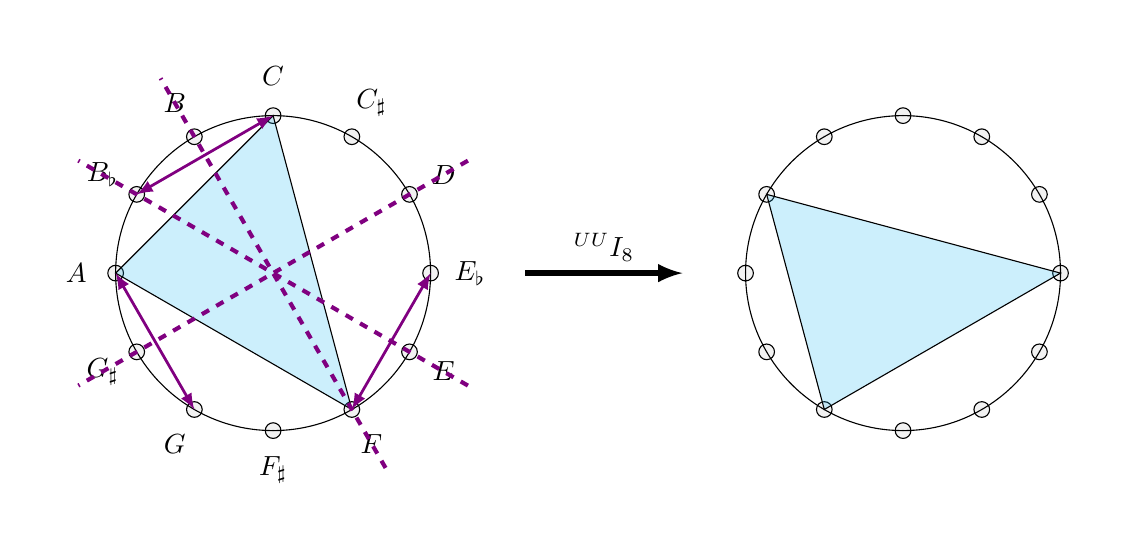
\begin{tikzpicture}
%% red, green, blue, cyan , magenta, yellow, black, gray, darkgray, lightgray, brown, lime, olive, orange, pink, purple, teal, violet and white.
	\draw (-5,0) circle[radius=2.0]; 
	\foreach \i in {0,...,11} {
		\node[circle,draw=black,fill=black, fill opacity = 0.05, inner sep=1pt, minimum size=3pt] (A\i) at ({-5.0+2.0*sin(\i*30)},{2.0*cos(\i*30)}) {.};
	}

	% Inversion nodes
	\foreach \i in {0,...,23} {
		\node (INV\i) at ({-5.0+3.0*sin(\i*15)},{3.0*cos(\i*15)}) {};
	}

	\foreach \i / \name in {0/$C$,1/$C_\sharp$,2/$D$,3/$E_\flat$,4/$E$,5/$F$,6/$F_\sharp$,7/$G$,8/$G_\sharp$,9/$A$,10/$B_\flat$,11/$B$} {
		\node (N\i) at ({-5.0+2.5*sin(\i*30)},{2.5*cos(\i*30)}) {\name};
	}
	\draw[ draw=black, fill=cyan, fill opacity=0.2] (A5.center) -- (A9.center) -- (A0.center) --cycle;
	\draw[ -, dashed, line width=1.5, color=violet] (INV8) to (INV20); 
	\draw[ -, dashed, line width=1.5, color=violet] (INV4) to (INV16); 
	\draw[ -, dashed, line width=1.5, color=violet] (INV10) to (INV22); 
	\draw[ latex-latex, line width=1.0, color=violet] (A5.center) to (A3.center);
	\draw[ latex-latex, line width=1.0, color=violet] (A0.center) to (A10.center);
	\draw[ latex-latex, line width=1.0, color=violet] (A9.center) to (A7.center);
	
	%%
	\draw[->,>=latex, color=black,line width=2,] (-1.8,0.0) to node[above,midway]{${}^{UU}I_8$} (0.2,0) ;
	%%
		
	\draw (3,0) circle[radius=2.0]; 
	\foreach \i in {0,...,11} {
		\node[circle,draw=black,fill=black, fill opacity = 0.05, inner sep=1pt, minimum size=3pt] (C\i) at ({3+2.0*sin(\i*30)},{2.0*cos(\i*30)}) {.};
	}
	\foreach \i in {0,...,11} {
		\node (D\i) at ({3+2.5*sin(\i*30)},{2.5*cos(\i*30)}) {};
	}
	\draw[ draw=black, fill=cyan, fill opacity=0.2] (C3.center) -- (C7.center) -- (C10.center) --cycle;
\end{tikzpicture}
\end{center}
\caption{A complex chord transformation.}
\label{fig:chordtransformation_example}
\end{figure}

Defining this diagram with TikZ element by element is feasible, but one clearly sees the benefit in defining a general macro for drawing a twelve-tone circle, the names of the pitch classes, and any number of chords inside, along with the possibility of marking the transformations (usually inversions or transpositions).


\newpage

The following LaTeX/TikZ code is an attempt at defining such a macro in its most general form.

\begin{verbatim}
\usepackage{tikz}
\usetikzlibrary{positioning,calc}
\usetikzlibrary{arrows}
\usetikzlibrary{matrix}

\newcommand{\chordcircle}[6] {
  \draw (#1,#2) circle[radius=#3]; 
  \foreach \i in {0,...,11} {
    \node[circle,draw=black,fill=black,
              fill opacity = 0.05, inner sep=1pt,
              minimum size=3pt] 
              (#4_POINTS_\i) at ({#1+#3*sin(\i*30)},{#2+#3*cos(\i*30)}) {.};
  }
  \foreach \x in #5 {
    \foreach \i / \name in {0/$C$,1/$C_\sharp$,2/$D$,3/$E_\flat$,4/$E$,5/$F$,
                 6/$F_\sharp$,7/$G$,8/$G_\sharp$,9/$A$,10/$B_\flat$,11/$B$} {
      \node (#4_NAMES_\i) at ({#1+#3*1.2*sin(\i*30)},{#2+#3*1.2*cos(\i*30)}) {\name};
    }
  }
  % Inversion nodes
  \foreach \i in {0,...,23} {
    \node (#4_INV_\i) at ({#1+#3*1.5*sin(\i*15)},{#2+#3*1.5*cos(\i*15)}) {};
  }
	
  \foreach \chord/\thecolor in #6 {	
    \foreach \x [count=\xi from 0] in \chord {
      \node (p_\xi) at (#4_POINTS_\x) {};
    }
    \draw[ draw=black, fill=\thecolor, fill opacity=0.2] (p_0.center)
    \foreach \x [count=\xi from 0] in \chord {
      \ifnum \xi>0
        -- (p_\xi.center)
      \fi
    } --cycle;
  }
}
\end{verbatim}

\newpage

This code defines 
\begin{enumerate}
\item{a twelve-tone circle with nodes for each pitch class, whose center and radius can be defined (first three arguments). These nodes are named
\#4\_POINTS\_$i$ where \#4 is the fourth argument of the macro, and $i$ is their index (from 0 to 11).}
\item{a series of twelve nodes with pitch classes names, at 1.2*radius; their visibility can be switched on or off with the fifth argument. These nodes are named
\#4\_NAMES\_$i$ where \#4 is the fourth argument of the macro, and $i$ is their index (from 0 to 11).}
\item{a series of invisible nodes, which can be used for drawing inversions and transpositions. These nodes are named
\#4\_INV\_$i$ where \#4 is the fourth argument of the macro, and $i$ is their index (from 0 to 23).}
\end{enumerate}
This structure is shown in Figure \ref{fig:macro_structure}.

\begin{figure}[]
\begin{center}
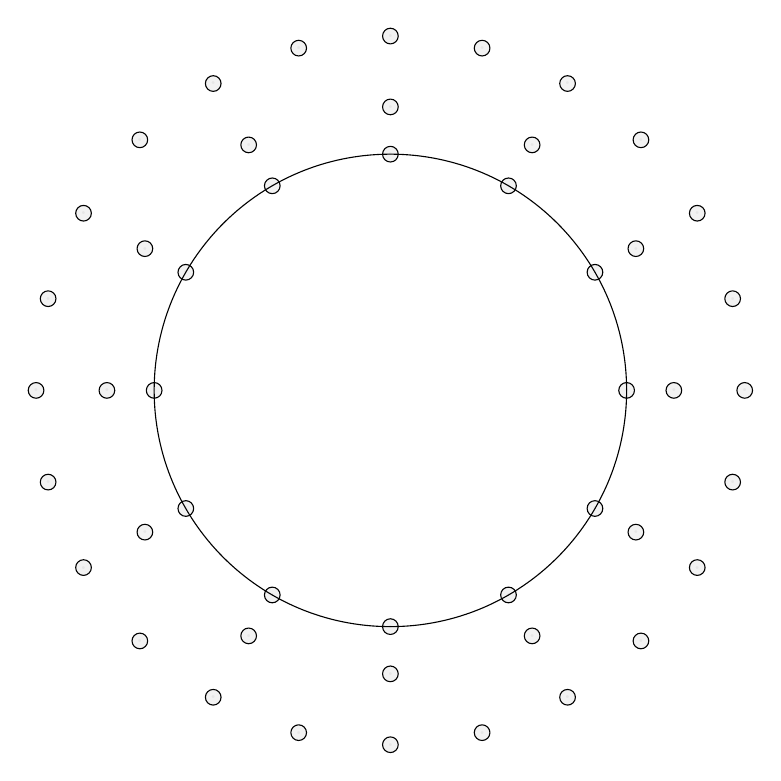
\begin{tikzpicture}[scale=0.75]
\draw (0,0) circle[radius=4]; 
  \foreach \i in {0,...,11} {
    \node[circle,draw=black,fill=black,fill opacity = 0.05, inner sep=1pt,minimum size=3pt] (A_POINTS_\i) at ({4*sin(\i*30)},{4*cos(\i*30)}) {.};
  }
  \foreach \i in {0,...,11} {
      \node[circle,draw=black,fill=black,fill opacity = 0.05, inner sep=1pt,minimum size=3pt] (A_NAMES_\i) at ({4*1.2*sin(\i*30)},{4*1.2*cos(\i*30)}) {.};
  }
  \foreach \i in {0,...,23} {
    \node[circle,draw=black,fill=black,fill opacity = 0.05, inner sep=1pt,minimum size=3pt] (A_INV_\i) at ({4*1.5*sin(\i*15)},{4*1.5*cos(\i*15)}) {.};
  }
\end{tikzpicture}
\end{center}
\caption{Structure of the diagram of nodes created by the macro.}
\label{fig:macro_structure}
\end{figure}

\newpage

The syntax of this macro is as follows.

\begin{verbatim}
\definecolor{color1}{RGB}{r1,g1,b1}
\definecolor{color2}{RGB}{r2,g2,b2}
\chordcircle{center_X}{center_Y}{radius}{name}{pitch_class_names_flag}{
{
{list of pitch-class indices for chord 1}/color1,
{list of pitch-class indices for chord 2}/color2,
...
}
}
\end{verbatim}

The code below is a simple example of a single major chord, whose corresponding Figure is shown on the right.

\begin{tabular}{cp{6in}}
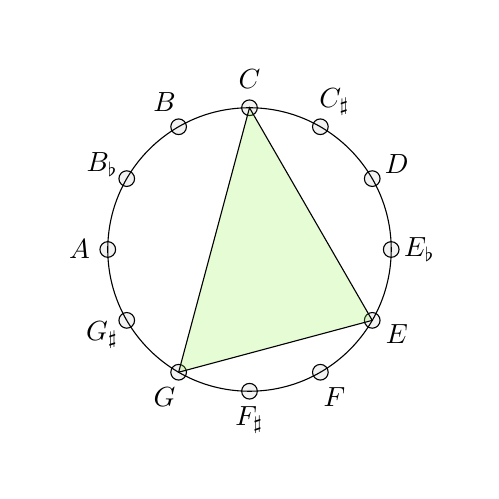
\begin{tikzpicture}[scale=0.45,baseline=50]
\definecolor{my_green}{RGB}{130,240,45}
\definecolor{my_yellow}{RGB}{255,200,0}
\chordcircle{0}{0}{4.0}{A}{1}{
{
{0,4,7}/my_green,
}
}
\end{tikzpicture}
&
\begin{verbatim}
\definecolor{my_green}{RGB}{130,240,45}
\chordcircle{0}{0}{4.0}{A}{1}{
{
{0,4,7}/my_green,
}
}
\end{verbatim}
\end{tabular}

The pitch classes names can be removed by passing nothing in the fifth argument.

\begin{tabular}{cp{6in}}
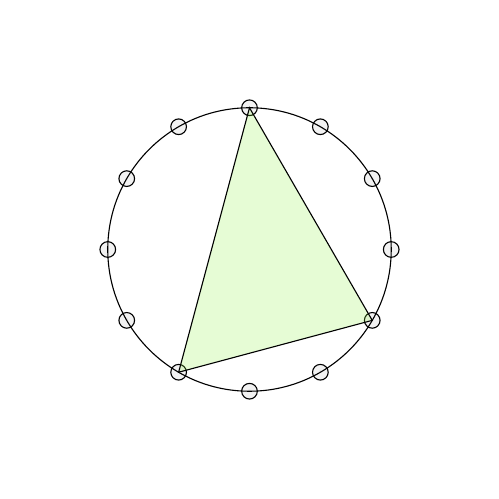
\begin{tikzpicture}[scale=0.45,baseline=50]
\definecolor{my_green}{RGB}{130,240,45}
\definecolor{my_yellow}{RGB}{255,200,0}
\chordcircle{0}{0}{4.0}{A}{}{
{
{0,4,7}/my_green,
}
}
\end{tikzpicture}
&
\begin{verbatim}
\definecolor{my_green}{RGB}{130,240,45}
\chordcircle{0}{0}{4.0}{A}{}{
{
{0,4,7}/my_green,
}
}
\end{verbatim}
\end{tabular}

\newpage

Multiple chords can be drawn, by adding them to the list of the sixth argument.

\begin{tabular}{cp{6in}}
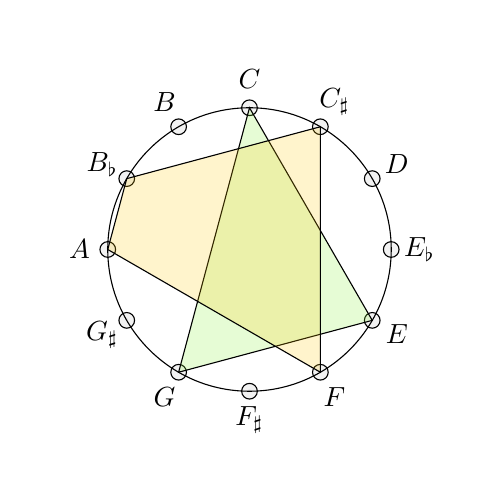
\begin{tikzpicture}[scale=0.45,baseline=50]
\definecolor{my_green}{RGB}{130,240,45}
\definecolor{my_yellow}{RGB}{255,200,0}
\chordcircle{0}{0}{4.0}{A}{1}{
{
{0,4,7}/my_green,
{1,5,9,10}/my_yellow,
}
}
\end{tikzpicture}
&
\begin{verbatim}
\definecolor{my_green}{RGB}{130,240,45}
\definecolor{my_yellow}{RGB}{255,200,0}
\chordcircle{0}{0}{4.0}{A}{1}{
{
{0,4,7}/my_green,
{1,5,9,10}/my_yellow,
}
}
\end{verbatim}
\end{tabular}

The pitch class nodes can be reused, for additional drawing.

\begin{tabular}{cp{6in}}
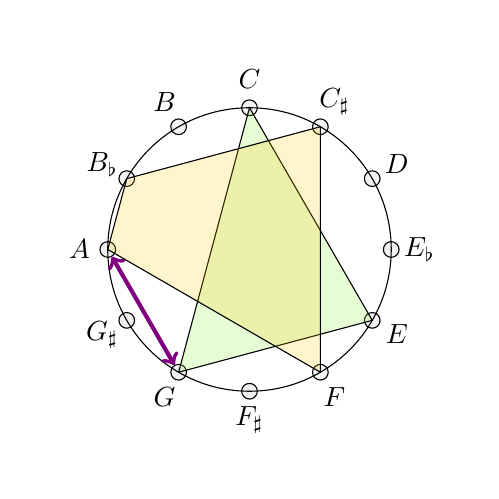
\begin{tikzpicture}[scale=0.45,baseline=60]
\definecolor{my_green}{RGB}{130,240,45}
\definecolor{my_yellow}{RGB}{255,200,0}
\chordcircle{0}{0}{4.0}{A}{1}{
{
{0,4,7}/my_green,
{1,5,9,10}/my_yellow,
}
}
\draw[ <->, line width=1.5, color=violet] (A_POINTS_7) to (A_POINTS_9); 
\end{tikzpicture}
&
\begin{verbatim}
\definecolor{my_green}{RGB}{130,240,45}
\definecolor{my_yellow}{RGB}{255,200,0}
\chordcircle{0}{0}{4.0}{A}{1}{
{
{0,4,7}/my_green,
{1,5,9,10}/my_yellow,
}
}
\draw[ <->, line width=1.5, color=violet]
    (A_POINTS_7) to (A_POINTS_9); 
\end{verbatim}
\end{tabular}

The transformation nodes can be used, for additional drawing. Below is an example
showing an inversion.

\begin{tabular}{cp{6in}}
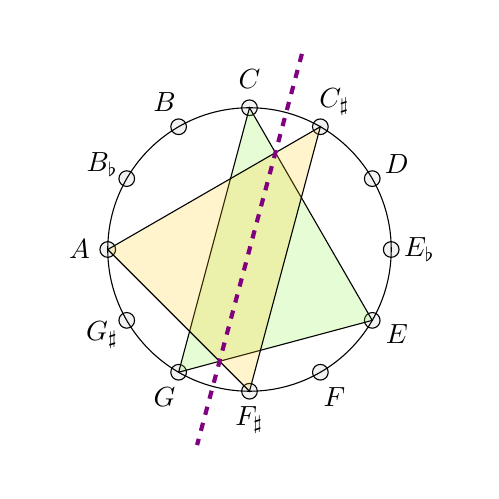
\begin{tikzpicture}[scale=0.45,baseline=60]
\definecolor{my_green}{RGB}{130,240,45}
\definecolor{my_yellow}{RGB}{255,200,0}
\chordcircle{0}{0}{4.0}{A}{1}{
{
{0,4,7}/my_green,
{1,6,9}/my_yellow,
}
}
\draw[ -, dashed, line width=1.5, color=violet]
    (A_INV_1) to (A_INV_13); 
\end{tikzpicture}
&
\begin{verbatim}
\definecolor{my_green}{RGB}{130,240,45}
\definecolor{my_yellow}{RGB}{255,200,0}
\chordcircle{0}{0}{4.0}{A}{1}{
{
{0,4,7}/my_green,
{1,6,9}/my_yellow,
}
}
\draw[ -, dashed, line width=1.5, color=violet]
    (A_INV_1) to (A_INV_13); 
\end{verbatim}
\end{tabular}

\newpage

The same nodes can be used to show transpositions.

\begin{tabular}{cp{6in}}
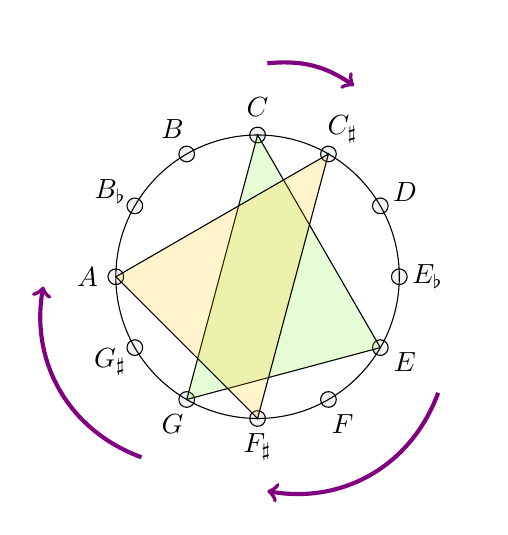
\begin{tikzpicture}[scale=0.45,baseline=90]
\definecolor{my_green}{RGB}{130,240,45}
\definecolor{my_yellow}{RGB}{255,200,0}
\chordcircle{0}{0}{4.0}{A}{1}{
{
{0,4,7}/my_green,
{1,6,9}/my_yellow,
}
}
\draw[ ->, line width=1.5, color=violet]
    (A_INV_0) to[bend left=20] (A_INV_2);
\draw[ ->, line width=1.5, color=violet]
    (A_INV_8) to[bend left=40] (A_INV_12);  
\draw[ ->, line width=1.5, color=violet]
    (A_INV_14) to[bend left=40] (A_INV_18);  
\end{tikzpicture}
&
\begin{verbatim}
\definecolor{my_green}{RGB}{130,240,45}
\definecolor{my_yellow}{RGB}{255,200,0}
\chordcircle{0}{0}{4.0}{A}{1}{
{
{0,4,7}/my_green,
{1,5,9,10}/my_yellow,
}
}
\draw[ ->, line width=1.5, color=violet]
    (A_INV_0) to[bend left=20] (A_INV_2); 
\draw[ ->, line width=1.5, color=violet]
    (A_INV_8) to[bend left=40] (A_INV_12);  
\draw[ ->, line width=1.5, color=violet]
    (A_INV_14) to[bend left=40] (A_INV_18);  
\end{verbatim}
\end{tabular}

\newpage

\section{Tonnetz diagrams}

Tonnetz diagrams are often used in neo-Riemannian music theory to show the $P$, $L$, and $R$ transformations and their successive application.
A typical Tonnetz has the topology of a torus, and can therefore be unfolded in 2D. The following code defines a macro for creating a Tonnetz diagram in TikZ, where the number of repeated cells can be defined in both directions.

\begin{verbatim}
\usepackage{tikz}
\usetikzlibrary{positioning,calc}
\usetikzlibrary{arrows}
\usetikzlibrary{matrix}

\newcommand{\tonnetzdiagram}[2] {
\foreach \i in {0,...,#1} {
  \foreach \j in {0,...,#2} {
    \node[] (Fs\i\j) at (0-1.5*\j+3.5*\i,0+\j*2.598+\i*0.866) {$F_\sharp$};
    \node[] (B\i\j) at (1-1.5*\j+3.5*\i,0+\j*2.598+\i*0.866) {$B$};
    \node[] (E\i\j) at (2-1.5*\j+3.5*\i,0+\j*2.598+\i*0.866) {$E$};
    \node[] (A\i\j) at (3-1.5*\j+3.5*\i,0+\j*2.598+\i*0.866) {$A$};	
    \draw[black, draw opacity=0.1, line width=0.5]
       (Fs\i\j.center) -- (B\i\j.center) -- (E\i\j.center) -- (A\i\j.center);		
    \node[] (D\i\j) at (0.5-1.5*\j+3.5*\i,-0.866+\j*2.598+\i*0.866) {$D$};
    \node[] (G\i\j) at (1.5-1.5*\j+3.5*\i,-0.866+\j*2.598+\i*0.866) {$G$};
    \node[] (C\i\j) at (2.5-1.5*\j+3.5*\i,-0.866+\j*2.598+\i*0.866) {$C$};
    \node[] (F\i\j) at (3.5-1.5*\j+3.5*\i,-0.866+\j*2.598+\i*0.866) {$F$};	
    \draw[black, draw opacity=0.1, line width=0.5]
       (D\i\j.center) -- (G\i\j.center) -- (C\i\j.center) -- (F\i\j.center);		
    \node[] (Bb\i\j) at (1-1.5*\j+3.5*\i,-2*0.866+\j*2.598+\i*0.866) {$B_\flat$};
    \node[] (Eb\i\j) at (2-1.5*\j+3.5*\i,-2*0.866+\j*2.598+\i*0.866) {$E_\flat$};
    \node[] (Ab\i\j) at (3-1.5*\j+3.5*\i,-2*0.866+\j*2.598+\i*0.866) {$A_\flat$};
    \node[] (Cs\i\j) at (4-1.5*\j+3.5*\i,-2*0.866+\j*2.598+\i*0.866) {$C_\sharp$};	
    \draw[black, draw opacity=0.1, line width=0.5]
       (Bb\i\j.center) -- (Eb\i\j.center) -- (Ab\i\j.center) -- (Cs\i\j.center);
			
    \draw[black, draw opacity=0.1, line width=0.5]
                (Fs\i\j.center) -- (D\i\j.center) -- (Bb\i\j.center);
    \draw[black, draw opacity=0.1, line width=0.5]
                (B\i\j.center) -- (G\i\j.center) -- (Eb\i\j.center);
    \draw[black, draw opacity=0.1, line width=0.5]
                (E\i\j.center) -- (C\i\j.center) -- (Ab\i\j.center);
    \draw[black, draw opacity=0.1, line width=0.5]
                (A\i\j.center) -- (F\i\j.center) -- (Cs\i\j.center);		
    \draw[black, draw opacity=0.1, line width=0.5]
                (D\i\j.center) -- (B\i\j.center);
    \draw[black, draw opacity=0.1, line width=0.5]
                (Bb\i\j.center) -- (G\i\j.center) -- (E\i\j.center);
    \draw[black, draw opacity=0.1, line width=0.5]
                (Eb\i\j.center) -- (C\i\j.center) -- (A\i\j.center);
    \draw[black, draw opacity=0.1, line width=0.5]
                (Ab\i\j.center) -- (F\i\j.center);			
  }
}
  
\foreach \i in {0,...,\the\numexpr#1-1\relax} {
  \foreach \j in {0,...,#2} {
    \draw[black, draw opacity=0.1, line width=0.5]
                (Cs\i\j.center) -- (Bb\the\numexpr\i+1\relax\j.center);
    \draw[black, draw opacity=0.1, line width=0.5]
                (F\i\j.center) -- (D\the\numexpr\i+1\relax\j.center);
    \draw[black, draw opacity=0.1, line width=0.5]
                (A\i\j.center) -- (Fs\the\numexpr\i+1\relax\j.center);
    \draw[black, draw opacity=0.1, line width=0.5]
                (A\i\j.center) -- (D\the\numexpr\i+1\relax\j.center);
    \draw[black, draw opacity=0.1, line width=0.5]
                (F\i\j.center) -- (Bb\the\numexpr\i+1\relax\j.center);
  }
}
	 
\foreach \i in {0,...,#1} {
  \foreach \j in {0,...,\the\numexpr#2-1\relax} {
    \draw[black, draw opacity=0.1, line width=0.5]
                (Fs\i\j.center) -- (Bb\i\the\numexpr\j+1\relax.center);
    \draw[black, draw opacity=0.1, line width=0.5]
                (B\i\j.center) -- (Eb\i\the\numexpr\j+1\relax.center);
    \draw[black, draw opacity=0.1, line width=0.5]
                (E\i\j.center) -- (Ab\i\the\numexpr\j+1\relax.center);
    \draw[black, draw opacity=0.1, line width=0.5]
                (A\i\j.center) -- (Cs\i\the\numexpr\j+1\relax.center);
    \draw[black, draw opacity=0.1, line width=0.5]
                (Fs\i\j.center) -- (Eb\i\the\numexpr\j+1\relax.center);
    \draw[black, draw opacity=0.1, line width=0.5]
                (B\i\j.center) -- (Ab\i\the\numexpr\j+1\relax.center);
    \draw[black, draw opacity=0.1, line width=0.5]
                (E\i\j.center) -- (Cs\i\the\numexpr\j+1\relax.center);
  }
}
\foreach \i in {0,...,\the\numexpr#1-1\relax} {
  \foreach \j in {1,...,#2} {
    \draw[black, draw opacity=0.1, line width=0.5] (Cs\i\j.center) 
    -- (Fs\the\numexpr\i+1\relax\the\numexpr\j-1\relax.center);
  }
}
}
\end{verbatim}

The cell (fundamental domain) being repeated by this macro is shown in yellow in the Figure below, wherein the Tonnetz diagram is generated by the command \verb|\tonnetzdiagram{2}{2};|. This cell corresponds to the coordinates $(0,0)$, while the coordinates of the repeated cells follow the pattern shown.

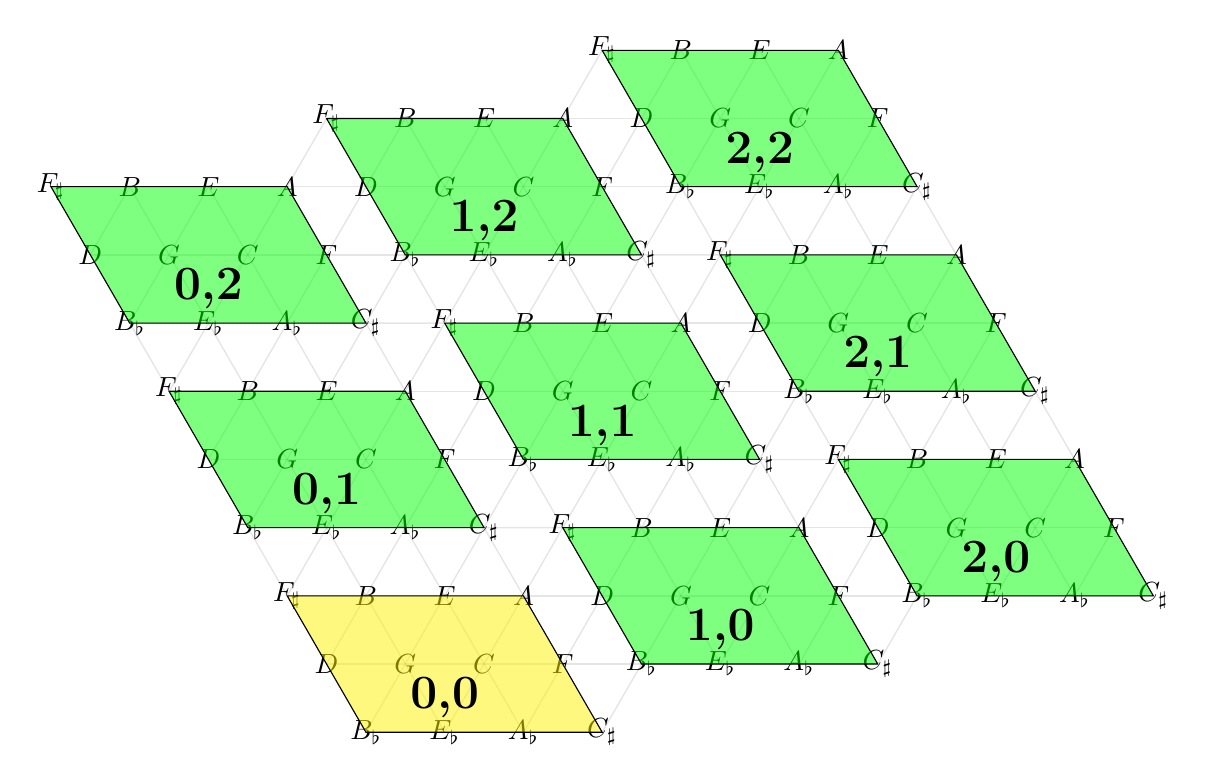
\begin{tikzpicture}[scale=1.0]
	\tonnetzdiagram{2}{2};
	\draw[draw=black, fill=yellow, fill opacity=0.5] (Fs00.center) -- (A00.center) -- (Cs00.center) -- (Bb00.center) --cycle;
	\node[] at ($(Bb00)!0.5!(Eb00)!0.5!(C00)$) {\textbf{\LARGE 0,0}};
	\draw[draw=black, fill=green, fill opacity=0.5] (Fs10.center) -- (A10.center) -- (Cs10.center) -- (Bb10.center) --cycle;
	\node[] at ($(Bb10)!0.5!(Eb10)!0.5!(C10)$) {\textbf{\LARGE 1,0}};
	\draw[draw=black, fill=green, fill opacity=0.5] (Fs20.center) -- (A20.center) -- (Cs20.center) -- (Bb20.center) --cycle;
	\node[] at ($(Bb20)!0.5!(Eb20)!0.5!(C20)$) {\textbf{\LARGE 2,0}};
	\draw[draw=black, fill=green, fill opacity=0.5] (Fs01.center) -- (A01.center) -- (Cs01.center) -- (Bb01.center) --cycle;
	\node[] at ($(Bb01)!0.5!(Eb01)!0.5!(C01)$) {\textbf{\LARGE 0,1}};
	\draw[draw=black, fill=green, fill opacity=0.5] (Fs11.center) -- (A11.center) -- (Cs11.center) -- (Bb11.center) --cycle;
	\node[] at ($(Bb11)!0.5!(Eb11)!0.5!(C11)$) {\textbf{\LARGE 1,1}};
	\draw[draw=black, fill=green, fill opacity=0.5] (Fs21.center) -- (A21.center) -- (Cs21.center) -- (Bb21.center) --cycle;
	\node[] at ($(Bb21)!0.5!(Eb21)!0.5!(C21)$) {\textbf{\LARGE 2,1}};
	\draw[draw=black, fill=green, fill opacity=0.5] (Fs02.center) -- (A02.center) -- (Cs02.center) -- (Bb02.center) --cycle;
	\node[] at ($(Bb02)!0.5!(Eb02)!0.5!(C02)$) {\textbf{\LARGE 0,2}};
	\draw[draw=black, fill=green, fill opacity=0.5] (Fs12.center) -- (A12.center) -- (Cs12.center) -- (Bb12.center) --cycle;
	\node[] at ($(Bb12)!0.5!(Eb12)!0.5!(C12)$) {\textbf{\LARGE 1,2}};
	\draw[draw=black, fill=green, fill opacity=0.5] (Fs22.center) -- (A22.center) -- (Cs22.center) -- (Bb22.center) --cycle;
	\node[] at ($(Bb22)!0.5!(Eb22)!0.5!(C22)$) {\textbf{\LARGE 2,2}};
\end{tikzpicture}


The named nodes can be accessed by the pitch class name followed by the coordinates. For example, this code

\begin{verbatim}
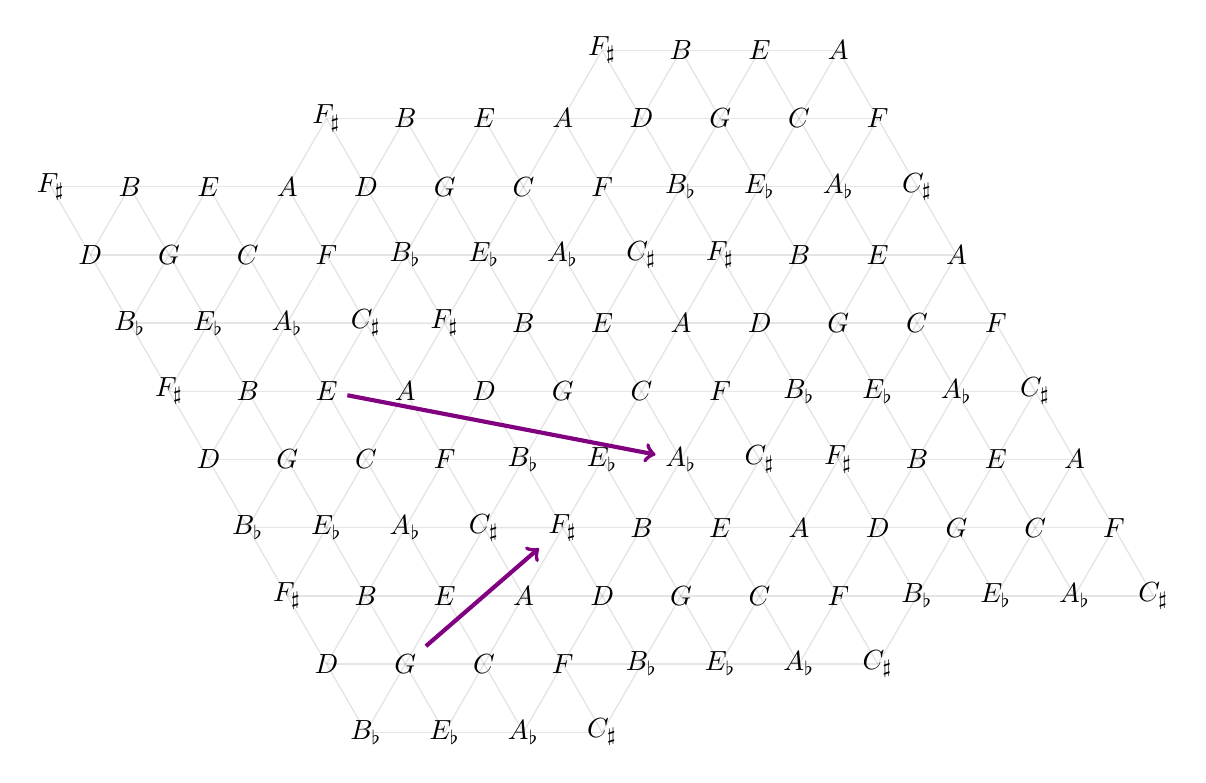
\begin{tikzpicture}[scale=1.0]
\tonnetzdiagram{2}{2};
\draw[ ->, line width=1.5, color=violet] (G00) to (Fs10);  
\draw[ ->, line width=1.5, color=violet] (E01) to (Ab11);  
\end{tikzpicture}

\end{verbatim}

generates the following Figure.

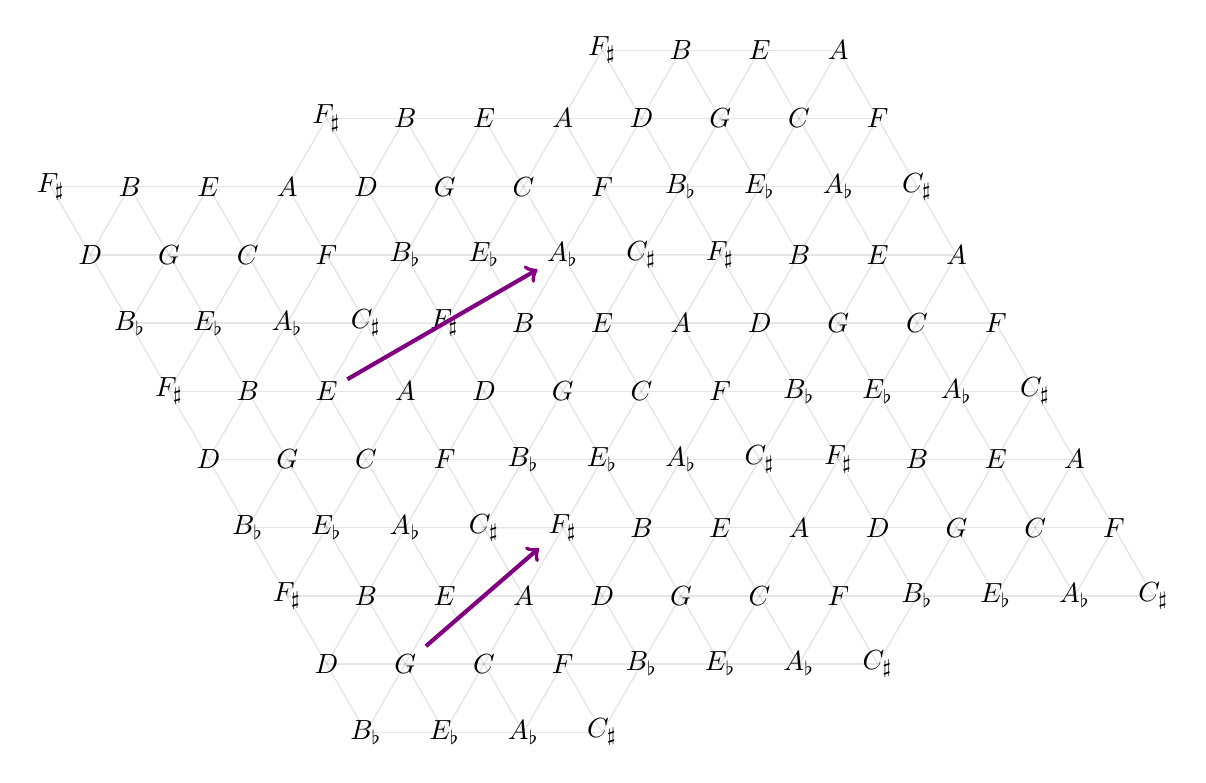
\begin{tikzpicture}[scale=1.0]
\tonnetzdiagram{2}{2};
\draw[ ->, line width=1.5, color=violet] (G00) to (Fs10);  
\draw[ ->, line width=1.5, color=violet] (E01) to (Ab12);  
\end{tikzpicture}

There are no nodes for the center of the triangles (major and minor chords) but they easily can be created from
the pitch class name nodes. For example, the code below

\begin{verbatim}
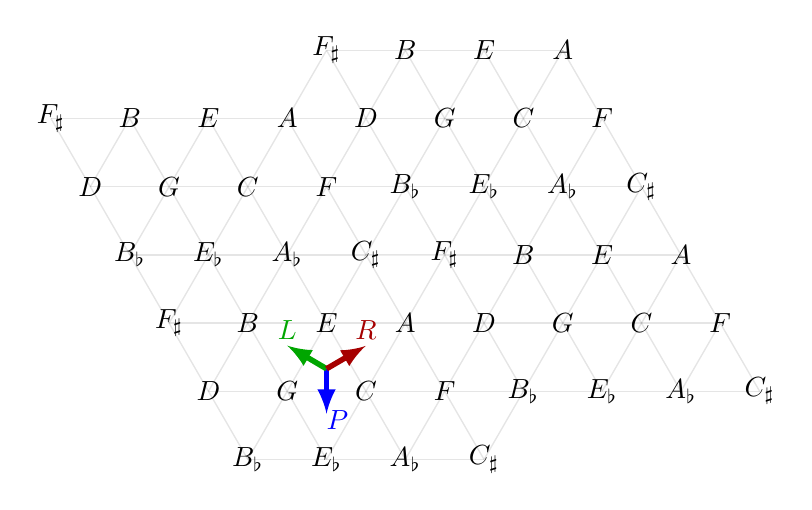
\begin{tikzpicture}[scale=1.0]
\tonnetzdiagram{1}{1};
\node[] (start) at ($(C00)!0.5!(G00)!0.33!(E00)$) {};
\node[] (endP) at ($(C00)!0.5!(G00)!0.33!(Eb00)$) {};
\node[] (endL) at ($(B00)!0.5!(E00)!0.33!(G00)$) {};
\node[] (endR) at ($(C00)!0.5!(E00)!0.33!(A00)$) {};
\draw[ -latex, line width=2, color=blue ] (start.center) to (endP.center); 
\draw[ -latex, line width=2, color=black!35!green] (start.center) to (endL.center); 
\draw[ -latex, line width=2, color=black!35!red] (start.center) to (endR.center); 
\node[color=blue] (Plabel) at ($(C00)!0.5!(Eb00)!0.15!(G00)$) {$P$};
\node[color=black!35!green] (Llabel) at ($(B00)!0.5!(E00)!0.1!(G00)$) {$L$};
\node[color=black!35!red] (Rlabel) at ($(A00)!0.5!(E00)!0.1!(C00)$) {$R$};
\end{tikzpicture}
\end{verbatim}

generates the following Figure, which shows the three basic neo-Riemannian operations starting from the C major chord.

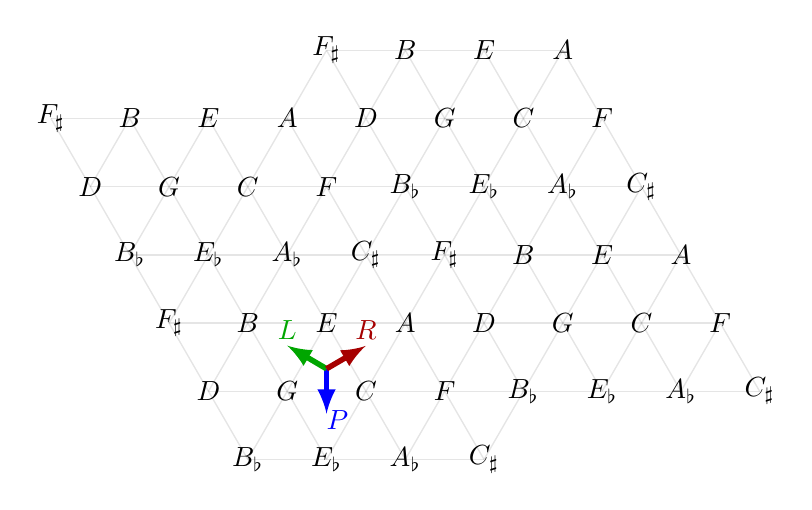
\begin{tikzpicture}[scale=1.0]
\tonnetzdiagram{1}{1};
\node[] (start) at ($(C00)!0.5!(G00)!0.33!(E00)$) {};
\node[] (endP) at ($(C00)!0.5!(G00)!0.33!(Eb00)$) {};
\node[] (endL) at ($(B00)!0.5!(E00)!0.33!(G00)$) {};
\node[] (endR) at ($(C00)!0.5!(E00)!0.33!(A00)$) {};
\draw[ -latex, line width=2, color=blue ] (start.center) to (endP.center); 
\draw[ -latex, line width=2, color=black!35!green] (start.center) to (endL.center); 
\draw[ -latex, line width=2, color=black!35!red] (start.center) to (endR.center); 
\node[color=blue] (Plabel) at ($(C00)!0.5!(Eb00)!0.15!(G00)$) {$P$};
\node[color=black!35!green] (Llabel) at ($(B00)!0.5!(E00)!0.1!(G00)$) {$L$};
\node[color=black!35!red] (Rlabel) at ($(A00)!0.5!(E00)!0.1!(C00)$) {$R$};
\end{tikzpicture}




\section{Rhythmic canons}

A rhythmic canon consists in a motive and entries, both subsets of $\mathbb{Z}$. The following macro creates a TikZ diagram
showing a grid of regularly spaced beats. The abscissa corresponds to time ($\mathbb{Z}$), whereas the different entries of the canon
are shown vertically. A box is marked in black if a beat is played. The first and second argument determines the size of the grid.
The third argument is a list of integers corresponding to the motive, whereas the fourth argument is a list of integers corresponding to the entries.

\begin{verbatim}
\newcommand{\rhythmiccanon}[4] {
  \foreach \i in {0,...,#1} {
    \foreach \j in {0,...,#2} {
      \filldraw[draw=lightgray,fill=none] (\i,\j) rectangle (\i+1,\j+1);
    }
  }
  \foreach \i in #3 {
    \foreach \j [count=\cj] in #4 {
      \filldraw[draw=lightgray,fill=black] (\i+\j,\cj-1) rectangle (\i+\j+1,\cj);
    }
  }
}
\end{verbatim}

As an example, the following code

\begin{verbatim}
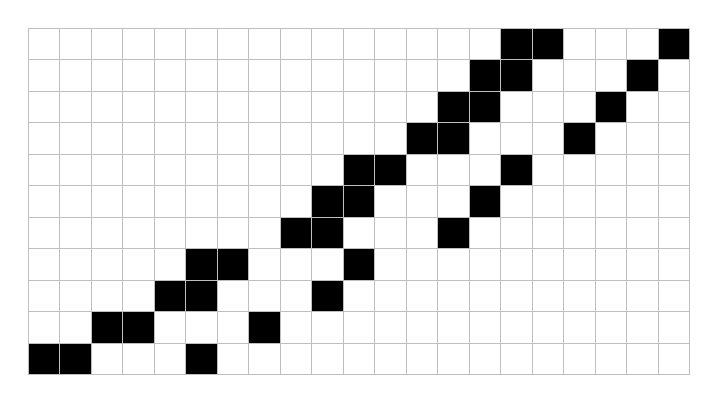
\begin{tikzpicture}[scale=0.4]
\rhythmiccanon{20}{10}{{0,1,5}}{{0,2,4,5,8,9,10,12,13,14,15}}
\end{tikzpicture}
\end{verbatim}

generates the following diagram.

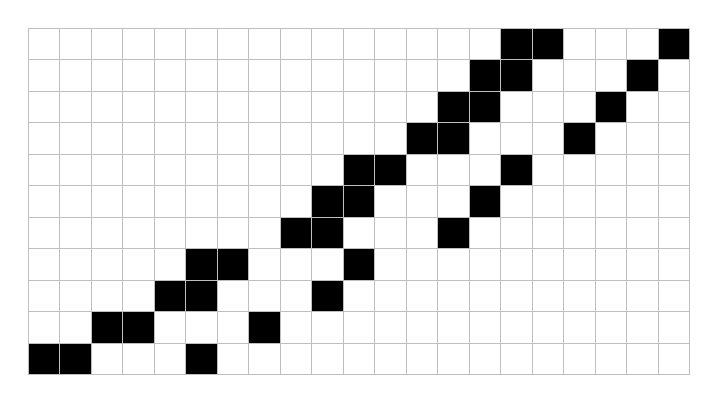
\begin{tikzpicture}[scale=0.4]
\rhythmiccanon{20}{10}{{0,1,5}}{{0,2,4,5,8,9,10,12,13,14,15}}
\end{tikzpicture}

\end{document}
